
\blank
\newpage

\section{Masked Language Models and Fine Tuning}

    I modelli linguistici tradizionali (Causal Language Models) sono autoregressivi: predicono la parola successiva basandosi solo sul contesto di sinistra (Left-to-right transformers).
    Al contrario, i \textbf{Bidirectional Transformer Encoders} (come BERT) sono progettati per vedere contemporaneamente sia il contesto sinistro che quello destro.
    
    L'architettura alla base è quella dell'Encoder del Transformer. A differenza dei modelli sequenziali classici, l'attenzione permette di mettere in relazione ogni token con tutti gli altri token della sequenza in parallelo.
    
    \begin{figure}[H]
        \centering
        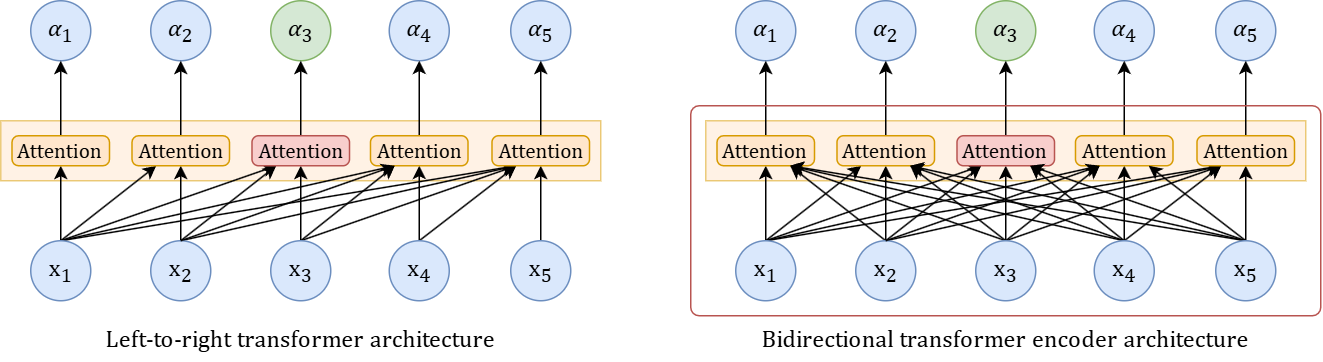
\includegraphics[width=1\linewidth]{imgs/schema_7_1.png}
        \label{fig:fig71}
    \end{figure}

        \subsection{BERT}
        
            BERT (Bidirectional Encoder Representations from Transformers) utilizza un'architettura a strati multipli di trasformatori. Le due versioni principali presentate sono:
            \begin{itemize}
                \item \textbf{BERT\textsubscript{BASE}}: 12 layer, 12 attention heads, 110M parametri.
                \item \textbf{BERT\textsubscript{LARGE}}: 24 layer, 16 attention heads, 304M parametri.
            \end{itemize}
            
            \paragraph{Input e Tokenizzazione.} BERT gestisce la complessità computazionale limitando l'input a 512 token (con embedding posizionali fissi).
            La tokenizzazione utilizza l'algoritmo \textbf{WordPiece} (una variante di BPE) con un vocabolario di circa 30.000 subwords.
            
            Rispetto al Byte Pair Encoding (BPE), l'algoritmo WordPiece addestra un semplice Language Model e, ad ogni passo, sceglie la fusione (merge) che accresce maggiormente la probabilità rispetto alla tokenizzazione (o ne minimizza la perplexity), invece di basarsi solo sulla frequenza.
            
            L'input finale per il modello è la somma di tre embedding distinti:
            \begin{itemize}
                \item \textbf{Token Embeddings}: la rappresentazione della subword.
                \item \textbf{Segment Embeddings}: per distinguere frasi diverse (es. Frase A vs Frase B).
                \item \textbf{Positional Embeddings}: per codificare la posizione nella sequenza.
            \end{itemize}
            
            \newpage

            \subsubsection{Pre-training di BERT}
                Il pre-training di BERT si basa su due task non supervisionati eseguiti contemporaneamente: Masked Language Modeling (MLM) e Next Sentence Prediction (NSP).
            
                \paragraph{Task 1: Masked Language Modeling (MLM)}                                
                Poiché il modello è bidirezionale, non può essere addestrato come un normale Language Model causale (che svelerebbe la parola successiva). Si utilizza un approccio "fill-in-the-blank" (Cloze task). In generale, il mascheramento è una forma di corruzione dell'input, che può avvenire tramite sostituzioni, riordinamenti o cancellazioni.

                \begin{figure}[H]
                    \centering
                    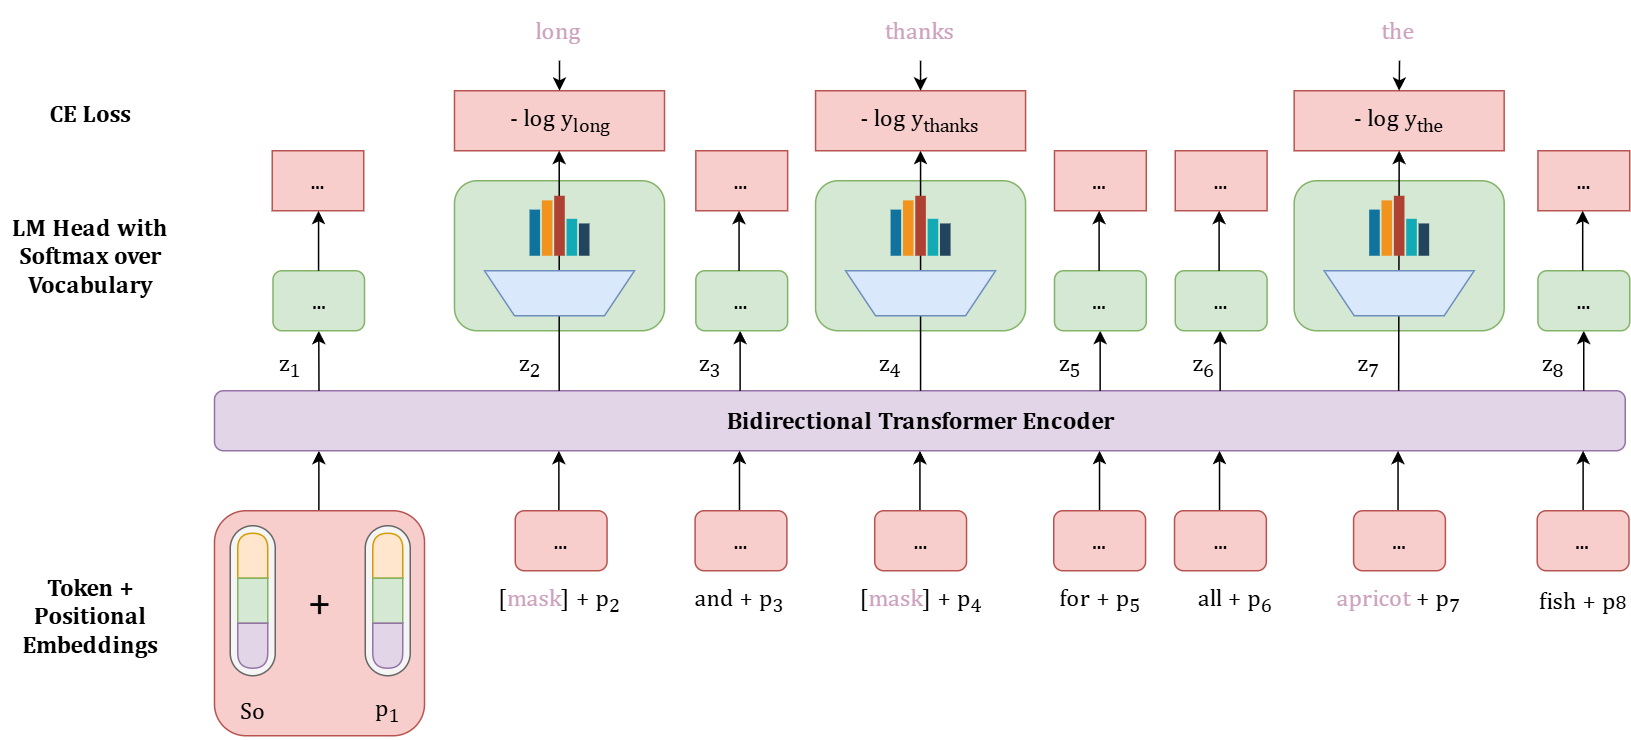
\includegraphics[width=1\linewidth]{imgs/schema_7_2.png}
                    \label{fig:fig72}
                \end{figure}

                \textbf{Strategia di Masking:}
                Il 15\% dei token di ogni sequenza viene campionato per l'apprendimento. Di questi token selezionati:
                \begin{itemize}
                    \item L'\textbf{80\%} viene sostituito con il token speciale \texttt{[MASK]}.
                    \item Il \textbf{10\%} viene sostituito con un token casuale.
                    \item Il \textbf{10\%} viene lasciato invariato.
                \end{itemize}
                
                \textbf{Funzione di Costo MLM:}
                La perdita è calcolata tramite Cross-Entropy solo sui token mascherati. Dato $h_i^L$ l'output dell'ultimo layer per il token $i$-esimo:
                $$ L_{MLM} = -\frac{1}{|M|}\sum_{i \in M} \log P(x_i | h_i^L) $$
                
                \newpage

                \paragraph{Task 2: Next Sentence Prediction (NSP)}
                Un altro tipo di addestramento per BERT è la Next Sentence Prediction. Molti task NLP (come Textual Entailment o QA) richiedono infatti di comprendere la relazione o la coerenza del discorso tra due frasi .
                L'input è formattato come: \texttt{[CLS] Frase A [SEP] Frase B [SEP]}.
                    
                \begin{figure}[H]
                    \centering
                    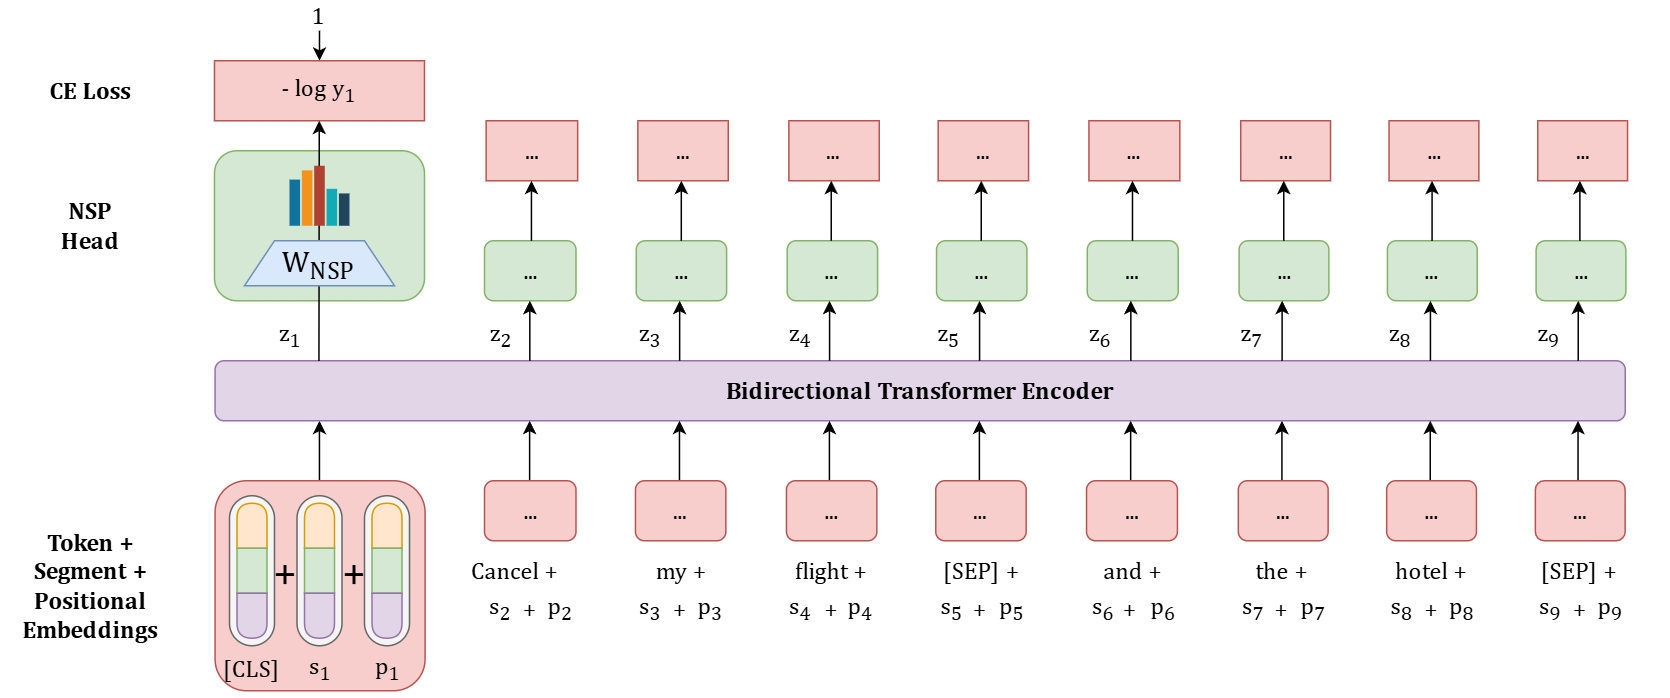
\includegraphics[width=1\linewidth]{imgs/schema_7_3.png}
                    \label{fig:fig73}
                \end{figure}

                Il modello deve predire in maniera binaria se la \textit{Frase B} segue logicamente la \textit{Frase A}:
                \begin{itemize}
                    \item 50\% dei casi: B è la frase successiva reale (Positive).
                    \item 50\% dei casi: B è una frase a caso dal corpus (Negative).
                \end{itemize}

                La predizione avviene usando l'embedding del token speciale \texttt{[CLS]}. Formalmente, l'output $y_i$ è calcolato come:
                $$ y_i = \text{softmax}(h_{CLS}^L W_{NSP}) $$
                dove $W_{NSP} \in \mathbb{R}^{2 \times d_h}$. La loss totale del modello durante il pre-training diviene quindi :
                $$ L_{TOT} = L_{NSP} + L_{MLM} $$

                \subsubsection{Embedding Contestuali}
                A differenza degli embedding statici (es. Word2Vec) dove ogni parola ha un vettore fisso che rappresenta il significato del \textit{tipo} di parola, gli embedding generati da MLM sono \textbf{contestuali}; vettori che rappresentano il significato della specifica \textit{istanza} della parola nel proprio contesto . Spesso il contextual embedding ottimale si ottiene facendo la media degli stati nascosti negli ultimi quattro layer del modello.

                Questo permette di gestire la \textbf{polisemia} (es. il termine inglese "die" come verbo morire o come dado da gioco) . Un'applicazione diretta è il \textbf{Word Sense Disambiguation (WSD)}. Ad esempio, tramite un algoritmo 1-nearest neighbour, si calcola l'embedding di un senso ($v_s$) come media dei token contestuali ($v_i$), e si assegna alla parola target $t$ il senso che massimizza la \textit{cosine similarity} :
                $$ v_s = \frac{1}{n}\sum_{i} v_i $$
                $$ sense(t) = \text{argmax}_{s \in senses(t)} \text{cosine}(t, v_s) $$

        \newpage

        \subsection{Fine-Tuning}
        Il "Transfer Learning" avviene adattando il modello pre-addestrato a task specifici aggiungendo un livello finale (head).
        
        \subsubsection{Classificazione di Sequenze}
        Si utilizza l'output del token \texttt{[CLS]} come rappresentazione dell'intera frase. Si aggiunge un layer denso $W_C$:
        $$ y = \text{softmax}(h_{CLS}^L W_C) $$
        
        \begin{figure}[H]
            \centering
            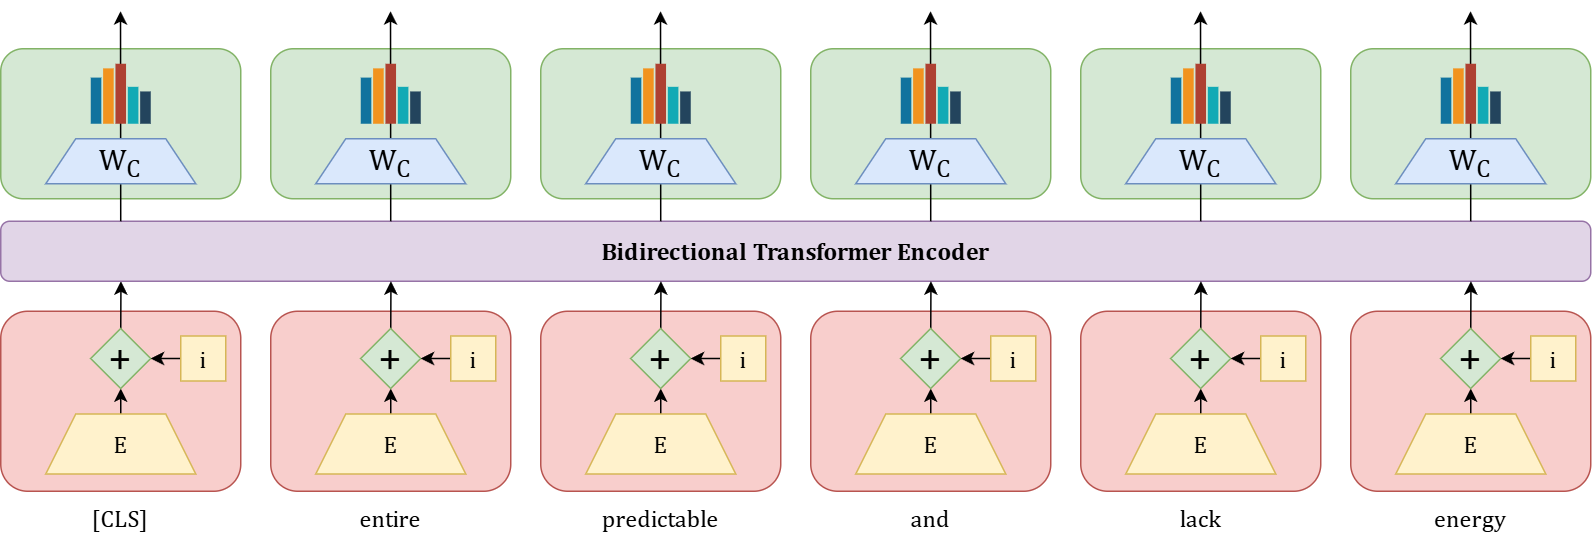
\includegraphics[width=1\linewidth]{imgs/schema_7_4.png}
            \label{fig:fig74}
        \end{figure}

        \textbf{Nota}: Le architetture BERT-based sono ottime per compiti di analisi di sequenze; non è detto invece che i Large Language Models (LLM) generativi arrivino alle stesse performance attuali su questi specifici task di classificazione.
        
        \subsubsection{Sequence Labeling (es. NER)}
        Per task come il Named Entity Recognition, serve una decisione per ogni token.
        Si applica un classificatore $W_K$ su ogni output $h_i^L$. Poiché WordPiece spezza le parole, solitamente si usa la predizione del primo sub-word token per etichettare l'intera parola.
        
        \subsection{Varianti di BERT}
            
            \begin{itemize}
            
                \item\textbf{SpanBERT}
                In SpanBERT si ha una nuova loss (negativa), che viene appresa a parte dalla rete e poi viene sommata alla MLM.
                Così facendo il modello impara a classificare interi pezzi di frasi (span) e non solo singoli token. Il processo viene effettuato per ciascuna parola mascherata all'interno dello span.
                
                \item\textbf{RoBERTa (Robustly Optimized BERT)}
                Sviluppato da Facebook, introduce ottimizzazioni chiave:
                \begin{itemize}
                    \item \textbf{Dynamic Masking}: la maschera cambia ogni volta che una sequenza viene passata al modello.
                    \item Rimuove il task NSP (Next Sentence Prediction).
                    \item Addestrato su una quantità di dati molto maggiore.
                \end{itemize}
                
                \item\textbf{XLM e Modelli Multilingua}
                \textbf{XLM (Cross-lingual Language Model)} introduce il \textit{Translation Language Modeling (TLM)}: l'input contiene una frase in lingua A e la traduzione in lingua B concatenate. Il modello fa attention su entrambe le lingue per predire le maschere, imparando allineamenti cross-lingua.
            
            \end{itemize}